\documentclass[11pt]{article}
\usepackage{graphicx}
%\usepackage{mystyle}
\usepackage{textcomp}
\usepackage[usenames,dvipsnames]{xcolor}

\def\al{\alpha}
\def\ks{{\sc KaSim}}
\def\ttt#1{\texttt{\textcolor{blue}{#1}}}
\def\mtt#1{{\tt{\color{blue} #1}}}
\def\at{\ @\ }
\def\lab#1{\hbox{\ttt{\color{Plum}\textquotesingle #1\textquotesingle}}}
\def\int{{\scriptstyle\sim}}
\def\mod{\hbox{\tt\$}}

\def\Krule#1#2#3{\color{blue}\mtt{{\color{blue}\lab{#1}\ #2\ @\ #3}}}
\def\Kndec#1#2#3{\color{blue}\mtt{\hbox{\color{blue}\tt\%}#1:\ \lab{#2}\ #3}}
\def\Kadec#1#2{\color{blue}\mtt{\hbox{\color{blue}\tt\%}#1:\ #2}}
\def\Kar{\ {\scriptstyle\tt-\! >}\ }
\def\Kbar{\ {\scriptstyle\tt<\!-\! >}\ }
\def\Kcom#1{\hbox{\tt \##1}}
\def\Kfile#1{\hbox{\ttt{\textquotesingle\textquotesingle #1\textquotesingle\textquotesingle}}}


\begin{document}

\title{Polymers in Kappa: a tutorial}
\author{Jean Krivine \thanks{Jean.Krivine@pps.univ-paris-diderot.fr}\\\\ PPS lab. CNRS and Univ. Paris Diderot - UMR 7126}
\date{}
\maketitle
\section{Introduction}
In this tutorial we want to study the question of how a protein with a specific DNA interaction capability, such as a transcription factor, is able to (rapidly) find its target on DNA. Indeed if one considers that a DNA strand has the order of $10^9$ base pairs, finding a particular sequence of a few nucleotides by colliding with DNA at random is rather unlikely. It has been argued~\cite{Dinant_etal09} that enzymes with specific DNA interactions combine 3D search (diffusion on the cytoplasm with random encounter with DNA) with 2D or 1D diffusion along the DNA to find their substrate (see Fig.~\ref{fig:search}). 
%%
%\begin{figure}[ht]
%\begin{center}
%\includegraphics[scale=0.80]{search.pdf}
%\caption{Two ways of finding a substrate for an enzyme with DNA binding capabilities.}\label{fig:search}
%\end{center}
%\end{figure}

In the present tutorial, we show that Kappa provides mechanistic ways to model such systems. We will model both 2D and 3D diffusion of a repair enzyme that is looking for U/G mismatches on DNA that arise after spontaneous hydrolytic deamination of cytosine bases. Deamination corresponds to the chemical transformation of a cytosine into a uracil. It is estimated that in a given genome, between 50 to 500 cytosines are deaminated per day~\cite{Krokan_etal02}. Several enzymes are known to have the capacity to recognize and initiate the repair of U/G mismatches, namely UNG, SMUG1, TDG and MBD4.  In the present tutorial we are not interested in the specific modeling of these enzymes and we will simply consider UDG (Uracil DNA Glycosylase) from the UNG family, the most frequent one. Roughly the repair process is the following: UDG, probably after a combination of sliding and 3D diffusion, reaches a U/G mismatch on DNA. It anchors strongly to it and excises the faulty U base, leaving an apurinic (AP) site: the DNA backbone with no nucleotide. The remaining part of the repair process is called \emph{Base Excision Repair} and involves several other enzymes that are able to put a cytosine back in the AP site, re-glue the DNA backbone and reform the C:G pairing. The model we will consider here stops after the intervention of UDG and we will treat the remaining of the repair as a (unbiological) single step.

There are three modeling challenges to raise here. The first one is of combinatorial nature: if one wishes to represent DNA sliding on a strand of size $n_D$, then one must take into account the fact all possible positions of the repair enzyme on DNA constitute a different molecular species, ie. there is the order of $2^{n_D}$ possible configurations. Also, if all the $n_C$ cytosine bases present on a DNA  may undergo a repair cycle of the form $C\rightarrow U\rightarrow AP\rightarrow C$, one must also consider the additional $3^{n_C}$ additional configurations of DNA. Essentially any approach which would try to enumerate (even on the fly) possible configuration would be doomed to fail. This first challenge is particularly well suited for Kappa, whose simulator has a cost per event that is independent of the number of possible molecular species the system may generate \cite{Dan_etal07b}. However using Kappa raises a second problem, inherent to the fact that space is abstracted away in this formalism. We will deal with this issue by showing one may use the structure link structure of DNA to model faithfully the distance between the enzyme on DNA and its substrates. Last, one has to face the question of running simulations on a realistic sample of DNA. We will see in the preliminary part of this tutorial, that one may use KaSim to generate meaningful initial conditions. 

\section{Preliminaries: generating initial conditions}

In this part of the tutorial one is interested in generating a Kappa representation of a double DNA strand with a random (and uniform) distribution of base pairs. 

\subsection{The choice of agent signatures} 
The obvious way to go would be to use one agent per nucleotide A,T,G,C or U. However a better choice is to consider a generic agent N (for nulceotide) which will allow us to specify rules which apply to all types of nucleotides (see Figure~\ref{fig:dna}). The signatures of N and UDG are declared in KaSim by the lines:
$$
\begin{array}{l}
\Kadec{agent}{N(e3,u,e5,o,i\int A\int T\int G\int C\int U\int AP)}\\
\Kadec{agent}{UDG(dbd)}
\end{array}
$$
where \texttt{e3} and \texttt{e5} are respectively the 3' and 5' ends of the nucleotides, \texttt{o} is its ``outter" face and \texttt{i} its ``inner" face. Note that this latter has 5 possible internal states which will be used to specialize the nucleotide to an A,T,G or C base, or an apurinic site. We equip UDG with a \emph{DNA binding domain} site called \texttt{dbd}. 
%%
%\begin{figure}[ht]
%\begin{center}
%\includegraphics[scale=0.65]{dna.pdf}
%\caption{An AG fragment of DNA (left) and a UDG enzyme bound to a G/U mismatch (right) in Kappa.}\label{fig:dna}
%\end{center}
%\end{figure}

\subsection{Growing DNA}
In a file \texttt{synth.ka} we put the signatures defined in the previous section, together with the following rules that will enable us to grow DNA strands:
$$
\color{blue}
\begin{array}{ll}
\tt\lab{growAT}& \tt N(i!0,e5),N(i!0,e3)\Kar\ \backslash\\ 
& \tt N(i!0,e5!1),N(i!0,e3!2),N(e3!1,i\int A!3),N(e5!2,i\int T!3)@\lab{kAT}\\
\tt\lab{growTA}& \tt N(i!0,e5),N(i!0,e3)\Kar\ \backslash\\ 
& \tt N(i!0,e5!1),N(i!0,e3!2),N(e3!1,i\int T!3),N(e5!2,i\int A!3)@\lab{kAT}\\
\tt\lab{growCG}& \tt N(i!0,e5),N(i!0,e3)\Kar\ \backslash \\ 
& \tt N(i!0,e5!1),N(i!0,e3!2),N(e3!1,i\int C!3),N(e5!2,i\int G!3)@\lab{kGC}\\
\tt\lab{growGC}& \tt N(i!0,e5),N(i!0,e3)\Kar\ \backslash \\ 
& \tt N(i!0,e5!1),N(i!0,e3!2),N(e3!1,i\int G!3),N(e5!2,i\int C!3)@\lab{kGC}
\end{array}
$$
Note that these rule may grow a new base pair provided there pre-exists in the mixture a base pair with a free 3':5' end. One solution would be to start from an initial state with such a pair. However a more elegant solution is seed the synthesis of DNA with the rules:
$$
\begin{array}{l}
\Krule{seedAT}{\Kar N(i\int A!0),N(i\int T!0)}{\lab{sAT}}\\
\Krule{seedGC}{\Kar N(i\int G!0),N(i\int C!0)}{\lab{sGC}}
\end{array}
$$
Recall that the convention adopted in \ks~is that agents that are created by a rule and whose interface is not fully specified, are completed using the signature of the agent\footnote{whenever a site that has possible internal states are not specified in the created agent, it receives the value indicated first in the signature.}.

In DNA, the ratio of GC pairs over AT ones is not evenly distributed. In the human genome the GC content (defined as $\frac{G+C}{A+T+G+C})$ is about 40\%. 
\\\\ \textbf{Question 1:}
Assuming that \lab{sAT}=\lab{kAT}, what should be the value of \lab{kGC} and \lab{sGC} in order to respect this ratio?
\\ \textbf{Answer:} The probability that rule $r$ applies is $\alpha(r)/\sum_i\alpha(r_i)$, where $\al(r_i)$ is the activity of rule $r_i$ defined as the number of matches of its left hand side, times its kinetic rate. Note that all the rules that introduce pairs of nucleotide have equal left hand sides. Therefore we can easily show that in order to respect the 40\% ratio of GC content, it suffices to set $\al(\lab{growAT})/\al(\lab{growGC})=\al(\lab{seedAT})/\al(\lab{seedGC})=1.5$. 

In \ks~variables can be declared by:
$$
\begin{array}{l}
\Kadec{var}{\lab{kGC}\ 1.0} \\
\Kadec{var}{\lab{kAT}\ 1.5\ *\ \lab{kGC}} \\
\Kadec{var}{\lab{sGC}\ 1.0} \\
\Kadec{var}{\lab {sAT}\ 1.5\ *\ \lab{sGC}} \\
\end{array}
$$
\\\\ \textbf{Question 2:} Given a state with $n$ strands of growing DNA. What is the likelihood that that a given strand is the next one to grow? 
\\\textbf{Answer:} Any strand has exactly two matches for the growing rules, one on the 3':5' end and the other on the 5':3' end. Therefore the probability that a given strand is the next to grow does not depend on its current length and is uniformly distributed. As a result one should expect that the $n$ strands will have in average the same length.
%%
\\\\ \textbf{Question 3:} One wishes to favor growing strands over creating new ones. What can we do for this?
\\\textbf{Answer:} an easy solution is to increase the ratio $\lab{kXY}/\lab{sXY}$. For instance we can set $\lab{kGC}=10$ and $\lab{sGC}=1$.

\subsection{Controlling the number of strands}

Instead of growing an undetermined number of DNA strands one may wish to restrict to \emph{exactly} $n$ strands. To do so, one needs to count how many times the seed rules have been applied. We will use \emph{tokens} to do this. We add the signature:
$$
\Kadec{token}{Cpt}
$$ 
and patch the seed rule as:
$$
\begin{array}{l}
\Krule{seedAT}{\Kar N(i\int A!0),N(i\int T!0)\ |\ 1:Cpt}{\lab{sAT}}\\
\Krule{seedGC}{\Kar N(i\int G!0),N(i\int C!0)\ |\ 1:Cpt}{\lab{sGC}}
\end{array}
$$
which tells \ks~to create 1 token \ttt{Cpt} at each application of a seed rule. Now the total number of seed applications can be accessed by \texttt{|Cpt|} (the number of tokens \texttt{Cpt}). One may then use the perturbation:
$$
\Kadec{mod}{|Cpt|=\hbox{$n$}\ do\ (\mod{UPDATE}\ \lab{sAT}\ 0.\ ;\ \mod{UPDATE}\ \lab{sGC}\ 0.)}
$$
which will turn off seeding new strands after $n$ applications. Note that since \lab{sAT}=0 if \lab{sGC}=0 it suffices to use the perturbation:
$$
\Kadec{mod}{|Cpt|=\hbox{$n$}\ do\ \mod{UPDATE}\ \lab{sGC}\ 0.}
$$


\subsection{Controlling the simulation}
In order to check that the GC content of the mixture is respected, one defines the following variables:
$$
\begin{array}{l}
\Kadec{var}{\lab{C}\ N(i\int C?)} \\
\Kadec{var}{\lab{G}\ N(i\int G?)} \\
\Kadec{var}{\lab{N}\ N()} \\
\end{array}
$$
which enable us to define the observable:
$$
\Kadec{obs}{\lab{GC content}\ (\lab{C}+\lab{G})/\lab{N}}
$$
Now one may run \ks~on the \ttt{synth.ka} file using the command:
\begin{center}\ttt{KaSim -i synth.ka -e 100000 -p 1000 -o data.out}\end{center}
which will generate one strand (if $n=1$ in the perturbation) of DNA of $10^5$ base pairs.

The content of \ttt{data.out} can be plotted using gnuplot for instance, and the result is given Fig.~\ref{fig:plot}.

%
\begin{figure}[ht]
\begin{center}
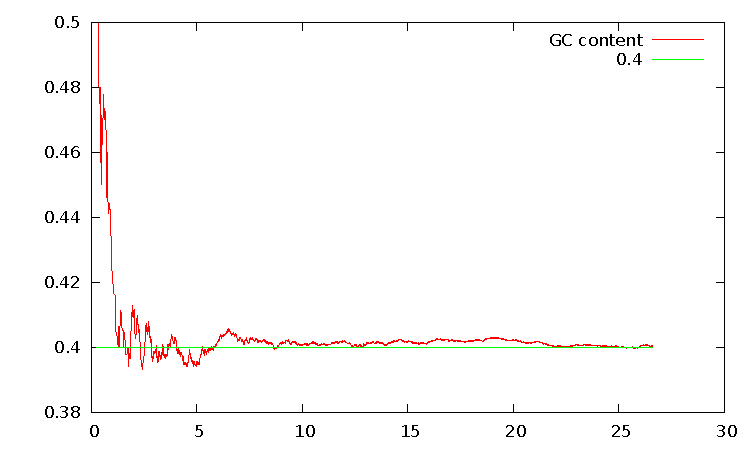
\includegraphics[scale=1]{plot.pdf}
\caption{Controlling the GC content of the synthesized DNA.}\label{fig:plot}
\end{center}
\end{figure}

\subsection{Visualizing and saving the final state}

Now that the model seems to be generating DNA, we need to be able to extract the final state of the simulation and use it as one of the input of our DNA repair model.

In order to save the state of a simulation one uses the perturbation:
$$
\Kadec{mod}{\lab{N}=\hbox{$n$}\ do\ \mod{SNAPSHOT}\ \Kfile{dna.ka}}
$$
which asks \ks~to save the state\footnote{The snapshot mechanism of \ks~will regroup all isomorphic species together and output each isomorphic class in an \ttt{\%init: $k$ $E$} declaration, where $k$ is the number of elements in the class, and $E$ the Kappa expression of one representative of the class.} whenever the number of nucleotides has reached $n$ (which makes a double strand DNA of length $n/2$). The state will be saved in the file \ttt{dna.ka} (which does not contain the signature of the agents). 

It is often convienent to generate a snapshot of the state that one may visualize instead of a plain Kappa file. To do so, one may tell \ks~to generate a dot format snapshot using the command:
$$
\Kadec{def}{\Kfile{dotSnapshots}\ \ \Kfile{true}}
$$
and the snapshot will be saved in the dot format file \ttt{dna.dot} instead. Dot format may be vizualised using the free software graphviz (and others). The snapshot of our model, using $n=20$ is given Fig.\ref{fig:snapshot}. 

%
\begin{figure}[htbp]
\begin{center}
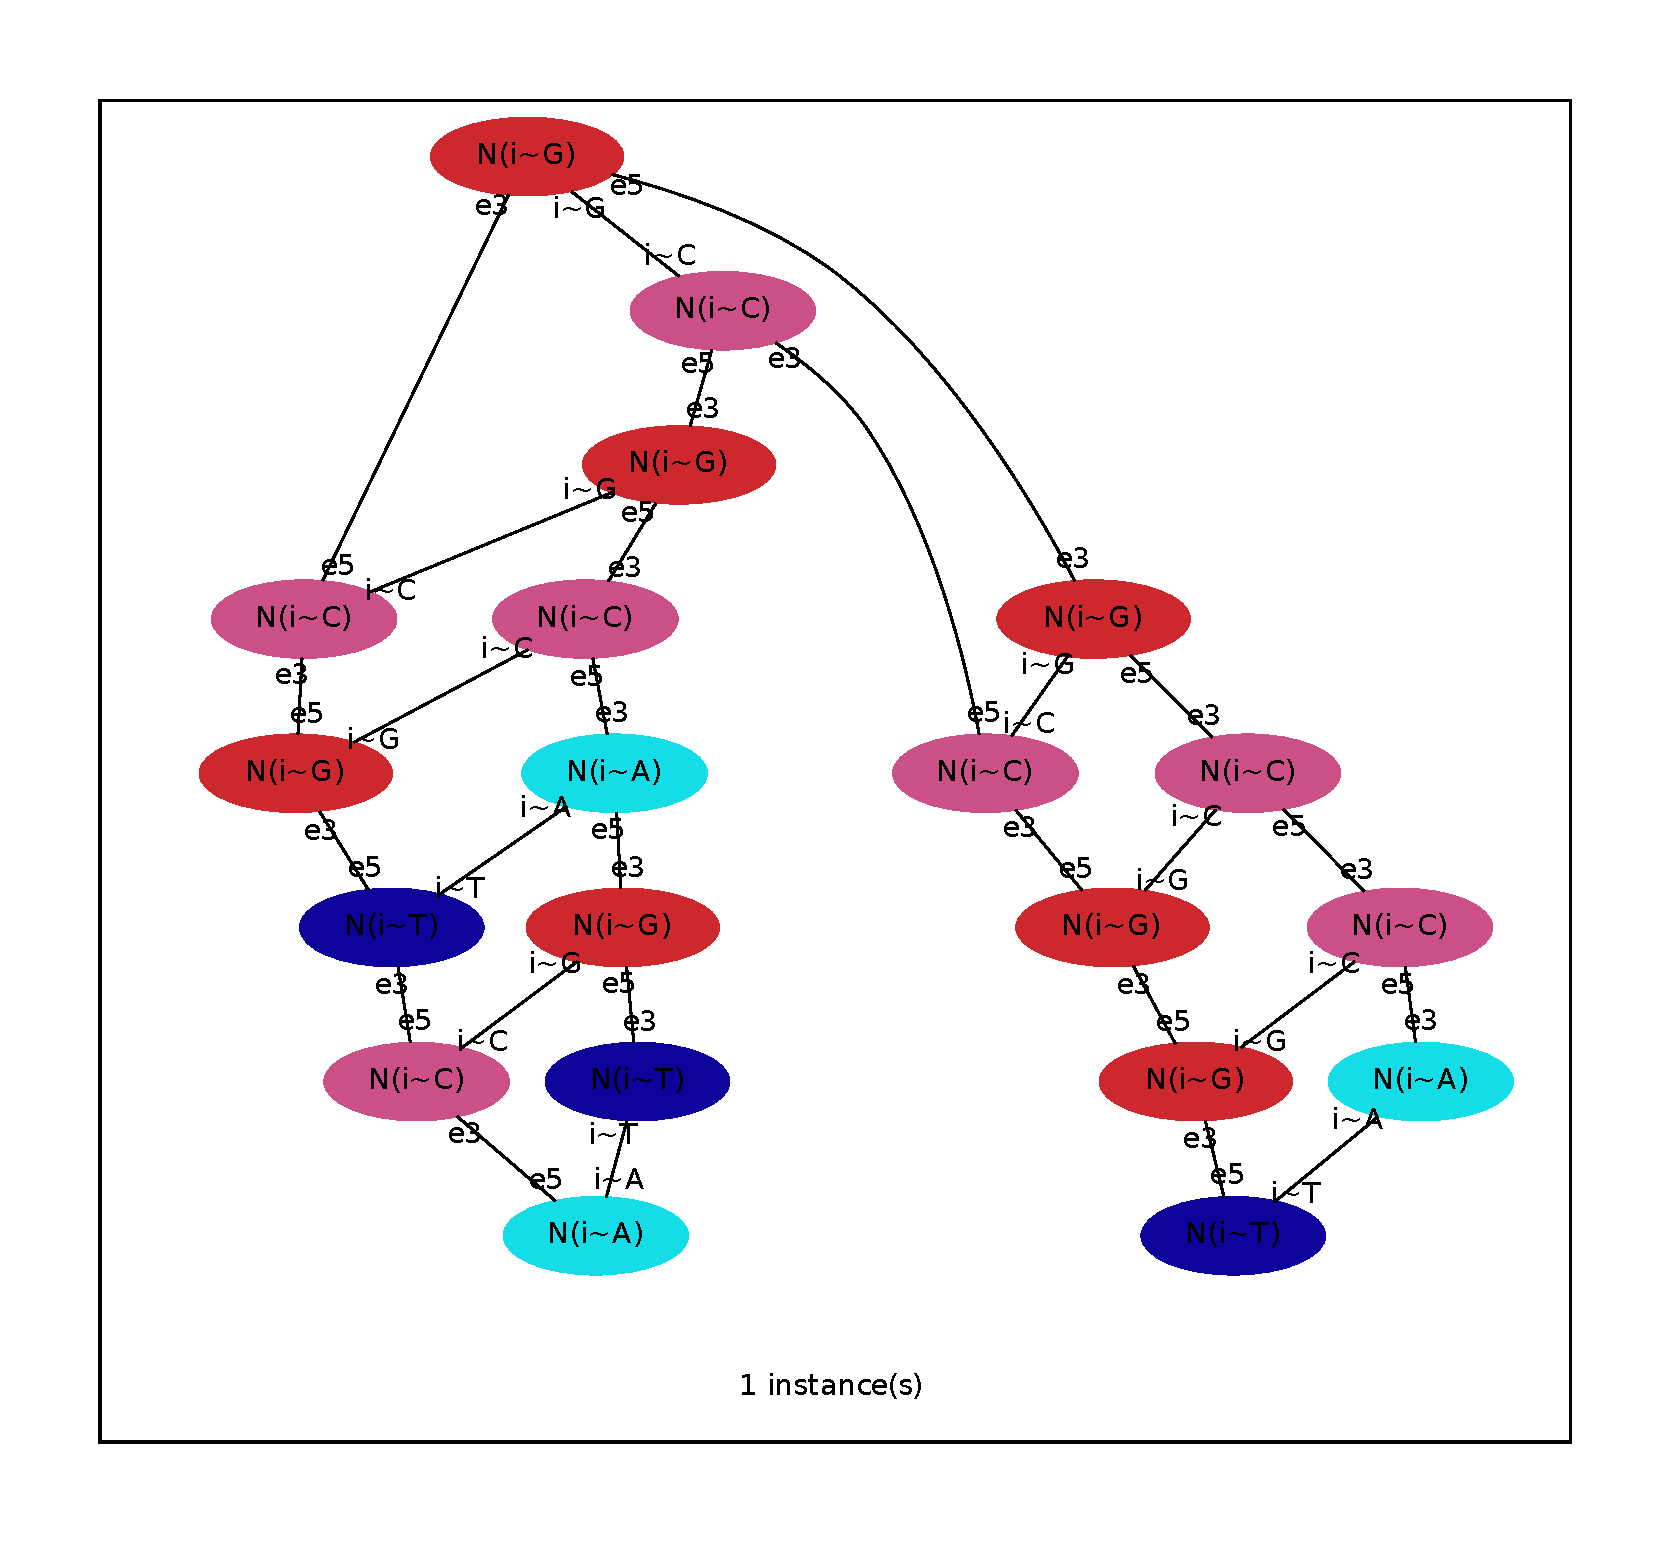
\includegraphics[scale=0.45]{snapshot.pdf}
\caption{Outputting the snapshot as a dot format enables one to visualize the species that are formed during a simulation, here an ACTGCGGCCA strand.}\label{fig:snapshot}
\end{center}
\end{figure}

\section{The DNA repair model}
We leave aside for now the \ttt{dna.ka} file generated at the previous state. We wish to represent in a different file, say \ttt{repair.ka}, the different step of the DNA repair model.

\subsection{Deamination}

\noindent\textbf{Question 1:} Assuming there are about 500 deamination events occuring each day in a mamalian cell (mamalian genomes have the order of $10^9$ base pairs). What should be the deamination rate of a single cytosine per second?
\\\textbf{Answer:} We saw that the GC content of a mamalian cell is 40\%. Hence there are about 20\% cytosines in a given genome, which makes $n_C=2*10^8$ cytosines. We have $n_C * k=500$ where $k$ is the deamination rate per cytosine per day. So the rate per second is: $k_{\mathit{deam}}=500/(n_C*24*60*60)=8.64*10^{-11} s^{-1}$. 

Obviously, this rate being very low, we will have to increase it a lot if we want to observe deamination in our small DNA strand.

The deamination rule is simply:
$$
\Krule{deamination}{\ N(i\int C!\_)\Kar N(i\int U)}{\lab{kdeam}}
$$
Note that the above rule is not atomic: we consider that the base pair is broken at the same time deamination occurs.

\subsection{3D diffusion and sliding}
We want to represent 3D diffusion and 2D sliding of UDG on DNA. 3D diffusion is going to be modelled by simple binding and unbinding of UDG to non specific nucleotides:
$$ 
\Krule{binding}{UDG(dbd),N(o)\Kbar UDG(dbd!1),N(o!1)}{\lab{kon}/\lab{V},\lab{koff}}
$$
where \lab{kon} is the constant association rate of UDG and DNA, \lab{V} is the volume in which our DNA strands floats (for instance the cell cytoplasm) and \lab{koff} is the dissociation rate. 
\vskip 0.25cm
\noindent\textbf{Question 1:} If we add no further rule, what would be the amount of UDG bound to DNA at steady state?
\\\textbf{Answer:} steady state will be reached whenever the probability of a binding event is equal to the probability of a dissociation, ie: $$U_{\mathit{free}}*N*k_{\mathit{on}}/V=k_{\mathit{off}}*U_{\mathit{bound}}$$ where $U_{\mathit{free}}$ and $U_{\mathit{bound}}$ are respectively the amount of free UDG and bound UDG, and $N$ is the number of nucleotides in the system (not the number of base pairs since UDG can bind on both Crick and Watson strands).

Remark that even with a very small $k_{\mathit{on}}$, most UDG will be bound because $N$ is big.

We know add the rules that model 2D diffusion of UDG on DNA:
$$
\begin{array}{lll}
 \lab{slide35} &\tt\color{blue} UDG(dbd!1),N(o!1,e3!2),N(o,e5!2)\Kbar \\
& \tt\color{blue} UDG(dbd!1),N(o,e3!2),N(o!1,e5!2)\ @\ \lab{kslide},\lab{kslide}
\end{array}
$$
Note that this rule is reversible and hence models diffusion in both 3'5' and 5'3' directions. 
\vskip .25cm
\noindent\textbf{Question 2:} Suppose that UDG lands on a particular spot on DNA, and suppose it slides during $n$ steps. What is the average distance the enzyme will cover? Suppose that a mismatch is located $k$ bases away from its landing spot. How many sliding steps would it take to reach it (assuming it doesn't unbind), in average.
\\\textbf{Answer:} The question is a trick and requires basic knowledge about random walks and ergodic processes to be answered. In a nutshell, the average distance the enzyme will cover is obviously 0 since the enzyme has an equal probablity to move to the left or to the right. However the random walk being ergodic, given enough time the enzyme will visit the whole strand. It takes in average $n$ steps to visit a nucleotide that is $\sqrt n$ bases away. So the mismatch can be found in average in $k^2$ steps.
%%  
%\vskip .25cm
%\noindent\textbf{Question 3:} It might be possible that the enzyme has the capacity to slide in one direction only (in the style of RNA polymerases). What difference would it make with respect to the model?
%\\\textbf{Answer:} Obviously UDG would find mismatches in the vicinity of its landing spot more quickly (assuming it may recognize U/G mismatch both from the U and G sides).  However this would induce a bias (TODO exact computation).

\subsection{Repair steps}

Whenever UDG finds a U/G mismatch it may remove the faulty U and leaves a apurinic site in its stead:
$$
\Krule{U removal}{UDG(dbd!1),N(o!1,i\int U)\Kar UDG(dbd),N(o,i\int AP)}{\lab{krepair}}
$$
\vskip 0.01cm
\noindent\textbf{Question 1:} Which other rules form a critical pair with the above one?
\\\textbf{Answer:} this rule will compete with both directions of the \lab{slide35} and with the unbinding of UDG from DNA. 

Finally the Base Excision Repair (BER) pathway enzymes (not modelled here) will put a cytosine in the apurinic site and form back the C:G base pair. We simply assume here that the repair is done spontaneously. 

The difficulty here is that in breaking the bond connecting both \ttt{i} sites of the paired nucleotides, we have lost the information about which nucleotide was opposite to the newly repaired one. To retrieve the information we need to exhibit a ``proof" in the left hand side of the rule that the G base is indeed opposite to the repaired base:
$$
\begin{array}{llll}
\lab{BER (1)}& \tt\color{blue} N(i\int AP,e5!1),N(e3!1,i!2)\ \backslash \\
& \tt\color{blue} N(i\int G\,\,\, ,e3!3),N(e5!3,i!2) \ \Kar \backslash \\
& \tt\color{blue} N(i\int C!0,e5!1),N(e3!1,i!2)\ \backslash \\
& \tt\color{blue} N(i\int G!0,e3!3),N(e5!3,i!2) \ @\ \lab{kber}
\end{array}
$$
Strictly speaking the above rule (we use indentation to suggests opposite bases) would not allow the repair of mismatches one the 5' end of the strand. To correct this we need the complementary rule that use the 3' direction to find the opposite base:
$$
\begin{array}{llll}
\lab{BER (2)}& \tt\color{blue} N(i\int AP,e3!1),N(e5!1,i!2)\ \backslash \\
& \tt\color{blue} N(i\int G\,\,\, ,e5!3),N(e3!3,i!2) \ \Kar \backslash \\
& \tt\color{blue} N(i\int C!0,e3!1),N(e5!1,i!2)\ \backslash \\
& \tt\color{blue} N(i\int G!0,e5!3),N(e3!3,i!2) \ @\ \lab{kber}
\end{array}
$$
However one should then deal with the fact that most mismatches will match both \lab{BER (i)} rules (ie. those which are not occuring on the end pairs of the strand) and hence will be repaired twice as fast, with rate $2*k_{\mathit{ber}}$. 
\vskip 0.25cm
\noindent\textbf{Question 1:} It seems one is forced to live with an approximation here: either neglecting the repair of a mismatch occuring on the 5' end and keep only the \lab{BER (1)} rule, or have the rate of repair of mismatches occurring on the 3' and 5' end be slower than the other mismatches. Is it a bad approximation? Can you compute the likelihood that a mismatch occurs exactly on the 3' or 5' end? 
\\\textbf{Answer:} Knowing that a deamination occurs, the probability that it concerns the 3' or the 5' end is the proba that the 3' end is a G:C pair and that a deamination occurrs here, plus the proba that the 5' end is a G:C pair and that a deamination occurs there, ie: $2*(0.4 / N_C)$.
\vskip 0.25cm
\noindent\textbf{Question 2:} Can you suggest an alternative representation of mismatches which would not induce any approximation in the repair rate?
\\\textbf{Answer:} Instead of deleting the bond in the \lab{deamination} rule, one could just maintain it and consider that it is only a symbolic link functionning as a pointer to the opposite strand. However the observable \ttt{N(i!\_)} would no longer enumerate the correct base pairs, and one would be forced to check the internal state as well. Other solutions are possible of course.

\section{Simulations}

\bibliography{fmb.bib}
\bibliographystyle{plain}
\end{document}
